\documentclass[UTF8,11pt,a4paper]{ctexart}
\usepackage[left=2.15cm,right=2.15cm,top=1.85cm,bottom=1.85cm]{geometry}
\usepackage{amsmath,amssymb,amsthm,mathtools,bm}
\usepackage{booktabs,array,tabularx}
\usepackage{graphicx,xcolor,hyperref,fancyhdr,enumitem,microtype,listings}

\definecolor{navy}{HTML}{17365D}
\definecolor{teal}{HTML}{0F6B73}
\definecolor{light}{HTML}{F3F6F8}
\hypersetup{colorlinks=true,linkcolor=navy,urlcolor=teal}
\pagestyle{fancy}
\fancyhf{}
\lhead{题三：QNM 谱不稳定性与可观测振铃}
\rhead{独立解答}
\cfoot{\thepage}
\setlength{\headheight}{14pt}
\setlist{nosep,leftmargin=2em}
\newtheorem{theorem}{定理}[section]
\newtheorem{proposition}[theorem]{命题}
\newtheorem{corollary}[theorem]{推论}
\theoremstyle{definition}
\newtheorem{remark}[theorem]{说明}
\newcommand{\E}{\mathcal E}
\newcommand{\M}{\mathcal M}
\newcommand{\cR}{\mathcal R}
\newcommand{\cS}{\mathcal S}
\newcommand{\Tr}{\operatorname{Tr}}
\newcommand{\norm}[1]{\lVert#1\rVert}
\newcommand{\ip}[2]{\langle#1,#2\rangle}
\newcommand{\dd}{\mathrm d}
\newcommand{\eps}{\varepsilon}
\newcommand{\om}{\omega}
\lstset{basicstyle=\ttfamily\small,backgroundcolor=\color{light},frame=single,
  columns=fullflexible,breaklines=true,showstringspaces=false}

\title{\bfseries 黑洞 QNM 的谱不稳定性\\究竟能否导致可观测振铃不稳定？\\[4pt]
\large 因果延迟、Jost 共振迁移与 source--detector 判据}
\author{独立推导与可复现计算}
\date{2026 年 9 月 23 日}

\begin{document}
\maketitle

\begin{abstract}
本文对题目给定的同一个 Regge--Wheeler 方程同时研究时域信号与解析延拓极点。
严格有限传播速度给出：外势垒对 $x_o=10$ 的最早影响时间是
$\tau_*(L)=2L-13$，此前两波形完全相同。Duhamel 展开说明一般情形下绝对误差为
$O(\eps)$、形状 mismatch 为 $O(\eps^2)$。simple QNM 的一阶位移含有
$\eps e^{2i\om_0L}$；由于高阶导数再产生 $L$，线性展开真正需要
$L\eps e^{2|\operatorname{Im}\om_0|L}\ll1$。在
$L=c\log(1/\eps)$ 下，这解释了谱重排与有限时间波形稳定可以并存。
本文证明了 $T=O(L)$ 窗口内的带对数误差界，但没有把全 $L$、全时间命题 (Q3c)
冒充为已证。两档时域网格及外部复标度 Jost 求根提供独立数值核验。
\end{abstract}

\section*{结论与证据等级}
\begin{center}
\begin{tabularx}{\textwidth}{>{\bfseries}p{2.8cm}X}
\toprule
已经证明 & 精确因果时刻 $2L-13$；有限时 Duhamel 展开及余项；
simple resonance 的一阶公式、双重极限的失效阈值；$T=O(L)$ 的波形稳定界。\\
精确低阶检验 & Jost 对数导数方程、Wronskian 导数与直接扰动后求根相互核验。\\
数值证据 & 两档网格的时域波形；两组外部复标度半径的 QNM；三组 $L$ 的位移系数。\\
尚未闭合 & (Q3c) 对全部 $L,T$ 的统一幂次界；临界窗口内完整新极点分支及其 residues；
真实探测器 PSD 下的可检测性。\\
\bottomrule
\end{tabularx}
\end{center}

\section{算符、初态与归一化}

写
\[
H_0=-\partial_x^2+V_0(x),\qquad H_{\eps,L}=H_0+\eps W_L,
\qquad W_L(x)=W(x-L).
\]
$V_0,W_L\ge0$，故二者在 $L^2(\mathbb R)$ 上的 Friedrichs 延拓均非负自伴。
初值记为 $f=CW$、$g=-CW'$。直接数值积分题给能量得到
\begin{equation}
E_0(C=1)=3.08614010142604,\qquad C=0.569235767826363.      \tag{1}
\end{equation}
该 $C$ 对所有 $(\eps,L)$ 固定。注意初值严格支撑在 $[-1,1]$，不是 Gaussian 尾部近似。

\section{A：先由因果传播求波形}

\subsection{精确 Duhamel 公式}

令
\[
S_0(t)=\frac{\sin(t\sqrt{H_0})}{\sqrt{H_0}},\qquad
\psi_0(t)=\cos(t\sqrt{H_0})f+S_0(t)g.
\]
差值 $u=\psi_{\eps,L}-\psi_0$ 满足零初值方程
$u_{tt}+H_0u=-\eps W_L\psi_{\eps,L}$，所以
\begin{equation}
u(t)=-\eps\int_0^tS_0(t-s)W_L\psi_{\eps,L}(s)\,\dd s.    \tag{2}
\end{equation}
迭代一次得到
\begin{align}
u(t)&=\eps u_1(t)+R_2(t),                                      \tag{3}\\
u_1(t)&=-\int_0^tS_0(t-s)W_L\psi_0(s)\,\dd s,                 \tag{4}\\
R_2(t)&=\eps^2\int_0^t\!\int_0^s
S_0(t-s)W_LS_0(s-r)W_L\psi_{\eps,L}(r)\,\dd r\dd s.          \tag{5}
\end{align}
因此观测量的一阶项是
\begin{equation}
h_1(t)=\partial_tu_1(t,x_o)
=-\partial_t\int_0^t\!\int_{L-1}^{L+1}
G_0^{\rm ret}(t-s;x_o,y)W(y-L)\psi_0(s,y)\,\dd y\dd s.        \tag{6}
\end{equation}

对任意固定 $T$，一维 Sobolev 迹估计与非负波动能量给出
\begin{equation}
\norm{\partial_tR_2(\cdot,x_o)}_{L^2(0,T)}
\le C_2\eps^2(1+T)^{9/2},                                    \tag{7}
\end{equation}
其中 $C_2$ 依赖 $V_0,W$ 的有限个有界导数和初值 Sobolev 范数，但因 $W_L$ 只是平移，
不依赖 $L$。幂 $9/2$ 不是最优值；它来自两次能量积分和一次点值迹估计。
式 (3) 的受控范围至少包括 $\eps(1+T)^2\ll1$。

\subsection{严格最早到达时间}

有限传播速度为 1。初始支撑的最右点是 1，势垒支撑的最左点是 $L-1$，观察者在 10。
任一受扰路径必须先从初态到势垒，再从势垒返回观察者，故
\begin{equation}
\tau_*(L)=\min_{y\in[L-1,L+1]}\{(y-1)+(y-10)\}=2L-13.      \tag{8}
\end{equation}
端点处 $W$ 平坦为零，因此等号时也没有贡献。

\begin{theorem}[精确因果相等]
对任意 $\eps$ 与 $L>12$，
\begin{equation}
h_{\eps,L}(t)=h_0(t),\qquad 0\le t\le2L-13.                 \tag{9}
\end{equation}
\end{theorem}

这不是“数值上很小”，而是双曲方程 domain of dependence 的精确陈述。

\subsection{两种观测量的首个非零阶}

设 $A_0=\int_0^\infty|h_0|^2\dd t>0$。由式 (3)、(7)，对固定 $T$，一般有
\begin{equation}
\E_{\eps,L}(T)=
|\eps|\frac{\norm{h_1}_{L^2(0,T)}}{\sqrt{A_0}}+O_T(\eps^2). \tag{10}
\end{equation}
令 $q=h_1|_{[0,T]}$、$f_T=h_0|_{[0,T]}$，并令
$q_\perp=q-\ip{q}{f_T}f_T/\norm{f_T}^2$。若两信号范数非零，则
\begin{equation}
\M_{\eps,L}(T)=
\frac{\eps^2}{2\norm{f_T}^2}\norm{q_\perp}^2+O_T(\eps^3). \tag{11}
\end{equation}
所以 generic 阶数分别是 $\eps$ 与 $\eps^2$。若 $T\le\tau_*$，二者前者精确为零，
后者在范数非零时也精确为零；若 $q=0$ 或 $q$ 与 $f_T$ 共线，则相应 leading coefficient
抵消。若任一截断信号范数为零，(Q3b) 按题意不定义。迟到回波除以某一时刻极小的背景振幅
可能很大，但这并不改变式 (10) 中以全程 $A_0$ 归一化的误差。

\section{B：同一系统的共振迁移}

\subsection{Jost--Wronskian 一阶公式}

令 $f_-(x,\om,\eps)$ 在左端满足 $e^{-i\om x}$，$f_+$ 在右端满足
$e^{+i\om x}$，并定义
\[
D(\om,\eps,L)=\mathcal W(f_-,f_+).
\]
QNM 是 $D$ 的零点而非 $L^2$ 本征值。若 $D(\om_0,0,L)=0$ 且
$\partial_\om D(\om_0,0,L)\ne0$，隐函数定理给出
\begin{equation}
\delta\om=-\eps\frac{\partial_\eps D(\om_0,0,L)}
{\partial_\om D(\om_0,0,L)}+O(\eps^2).                    \tag{12}
\end{equation}

等价地，在使 outgoing 波衰减的复标度轮廓 $\Gamma$ 上，以无共轭双线性型定义
\[
\mathcal N_0=\int_\Gamma u_0(x)^2\dd x,
\]
则
\begin{equation}
\delta\om=
\frac{\eps}{2\om_0\mathcal N_0}
\int_\Gamma W(x-L)u_0(x)^2\dd x+O(\eps^2).                \tag{13}
\end{equation}
这不是普通 $L^2$ Rayleigh 商。远区 $u_0=A_+e^{i\om_0x}[1+O(L^{-1})]$，故
\begin{equation}
\delta\om=\eps K_0e^{2i\om_0L}[1+O(L^{-1})]+\text{higher order},
\quad
K_0=\frac{A_+^2}{2\om_0\mathcal N_0}
\int_{-1}^1W(y)e^{2i\om_0y}\dd y.                         \tag{14}
\end{equation}

写 $\gamma=-\operatorname{Im}\om_0>0$。位移大小的小参数是
$\mu=|\eps K_0|e^{2\gamma L}$；但 $\om$ 导数作用于传播相位还会产生 $L$，
所以线性展开的相对误差由更严格的
\begin{equation}
\boxed{\eta=L|\eps K_0|e^{2\gamma L}\ll1}                 \tag{15}
\end{equation}
控制。若 $K_0=0$，需从下一非零阶开始，不能使用 generic 结论。

\subsection{双重极限与新分支}

取 $L=c\log(1/\eps)$。忽略不影响阈值的非零常数后，
\begin{equation}
\mu\asymp\eps^{1-2\gamma c},\qquad
\eta\asymp\log(1/\eps)\eps^{1-2\gamma c}.               \tag{16}
\end{equation}
因此：
\begin{itemize}
\item $c<(2\gamma)^{-1}$：$\eta\to0$，simple pole 的线性位移可靠且趋零；
\item $c=(2\gamma)^{-1}$：naive 一阶位移已是 $O(1)$，而 $\eta$ 发散，不能线性外推；
\item $c>(2\gamma)^{-1}$：固定 pole label 的微扰级数更强地失效，必须重求完整零点。
\end{itemize}

在原极点附近保留传播相位的最小 resummation 是
\[
z+a\eps e^{2i\om_0L}e^{2iLz}=0,
\qquad
z=-\frac{1}{2iL}W_n\!\left(2iLa\eps e^{2i\om_0L}\right). \tag{17}
\]
不同 Lambert 分支展示了为何“原来那个 pole”在失效区不再是稳健标签。

另一方面，两散射体的 cavity poles 满足
\begin{equation}
1-\mathcal R_{\rm BH}^{R}(\om)\mathcal R_{\rm b}^{L}(\om,\eps)
e^{2i\om L}=0.                                             \tag{18}
\end{equation}
对远离零频的频率，$\mathcal R_{\rm b}^{L}=\eps r_1+O(\eps^2)$，因而
\begin{equation}
\begin{aligned}
2\operatorname{Re}\om_nL+\arg(\mathcal R_{\rm BH}^{R}r_1)&=2\pi n+o(1),\\
\operatorname{Im}\om_n&=-\frac{1}{2L}\log\frac1{\eps|\mathcal R_{\rm BH}^{R}r_1|}
=-\frac1{2c}+o(1).
\end{aligned}                                               \tag{19}
\end{equation}
所以即使某个解析延拓分支不能继续用式 (12) 命名，仍可产生有限虚部高度的新共振列。
当 $c>(2\gamma)^{-1}$ 时，这一列比原 pole 更靠近实轴。

\subsection{为什么 pole 大变不迫使早期波形大变}

谱重排来自复频面上的 $e^{2\gamma L}$；时域却受式 (9) 的往返时间约束。
对任意固定 $K,c$，在 $L=c\log(1/\eps)$、$T\le KL$ 时，式 (2)--(7) 给出
\begin{equation}
\sup_{0\le T\le KL}\E_{\eps,L}(T)
\le C_{K,c}\eps[1+\log(1/\eps)]^{5/2}.                    \tag{20}
\end{equation}
故此窗口内波形仍趋于未扰动波形，即使复频极点的逐点微扰展开已经失效。

一个 pole 对实时间信号的贡献还乘以 residue、source overlap、detector overlap，并且必须等到
$\tau_*$ 后才出现。prompt response 由实轴高频 resolvent 决定；有限个 QNM 只可能描述某个中间
时间窗；Schwarzschild 的零频非解析性产生晚时 tail，最终不能被有限 pole sum 取代。

\section{C：统一稳定性命题的状态}

\subsection{source--detector resolvent 判据}

取单边变换 $\widehat\psi(\om)=\int_0^\infty e^{i\om t}\psi(t)\dd t$，则源项为
$s(\om)=g-i\om f$。令
$R_{\eps,L}(z)=(H_{\eps,L}-z^2)^{-1}$。因 $f(x_o)=0$，
\begin{equation}
\widehat h_{\eps,L}(\om)=-i\om\,\delta_{x_o}
R_{\eps,L}(\om+i0)s(\om).                                 \tag{21}
\end{equation}
resolvent identity 给出问题真正需要控制的量
\begin{align}
\Delta\widehat h(\om)
={}&i\om\eps\,\delta_{x_o}R_0(\om+i0)W_L
[I+\eps R_0(\om+i0)W_L]^{-1}R_0(\om+i0)s(\om).             \tag{22}
\end{align}
只要信号平方可积，Plancherel 表明 (Q3c) 等价于
\begin{equation}
\sup_{L\ge L_0}\int_{\mathbb R}|\Delta\widehat h(\om)|^2\dd\om
\le C\eps^{2\alpha}A_0.                                   \tag{23}
\end{equation}
式 (23) 同时固定了函数空间（实轴 $L^2_\om$）、允许扰动（题给的平移势垒）以及 source/detector。
一个未加权算符 pseudospectrum 很大，既不蕴含也不否定这个标量 sandwich bound。

\subsection{对 (Q3c) 的判定边界}

本文没有证明或推翻全 $L$、全时间的 (Q3c)。障碍不是有限时间连续依赖，而是需要对式 (22)
在零频 branch point 与可能的窄 cavity resonances 上作统一实轴积分估计。实频 unitarity 会限制
单频散射振幅，但不足以自动控制窄峰的总面积及其 source/detector residues。

因此最强已证结论是式 (20)。它特别蕴含：对任意 $\alpha<1$，该对数窗口内有
$\E=O(\eps^\alpha)$。要证伪 (Q3c)，下一步必须构造
$\eps_j\to0,L_j$，使式 (23) 左边保持正下界；只展示一个大 pole shift 不够。
要证明 (Q3c)，则需建立题给 $l=2$ 源在零频的 weighted limiting-absorption bound，并统一控制
$[I+\eps R_0W_L]^{-1}$ 的共振窄峰面积。

\section{数值核验}

\subsection{时域：两档网格}

使用二阶中心差分，粗细网格分别 $\Delta x=0.08,0.04$，CFL 为 0.45，计算域
$[-140,180]$，报告至 $T=100$。端点取齐次值；任何端点反射最早在 $T>289$ 才能返回观察者，
故报告窗口与边界因果隔离，而非把有限边界误称为精确 outgoing boundary。
表中为细网格；$L=5\log(1/\eps)$。

\begin{center}
\small
\begin{tabular}{ccccccc}
\toprule
$\eps$ & $L$ & $\tau_*=2L-13$ & $\E(100)$ & $\E/\eps$ & $\M(100)$ & 数值前驱最大值\\
\midrule
0.04 & 16.0944 & 19.1888 & 0.0084323 & 0.2108 & $3.5553\!\times10^{-5}$ & $1.70\!\times10^{-11}$\\
0.02 & 19.5601 & 26.1202 & 0.0041214 & 0.2061 & $8.4922\!\times10^{-6}$ & $4.63\!\times10^{-11}$\\
0.01 & 23.0259 & 33.0517 & 0.0020328 & 0.2033 & $2.0661\!\times10^{-6}$ & $7.43\!\times10^{-11}$\\
\bottomrule
\end{tabular}
\end{center}

粗细网格的 $\E(100)$ 相对差均小于 $0.18\%$。细网格的最后 20 个时间单位只占
$h_0$ 截断范数的 $4.13\times10^{-6}$；这量化了用 $T=100$ 近似分母的晚时截断误差。
数值显示 $\E\propto\eps$、$\M\propto\eps^2$，但不被提升为全参数定理。

\begin{center}
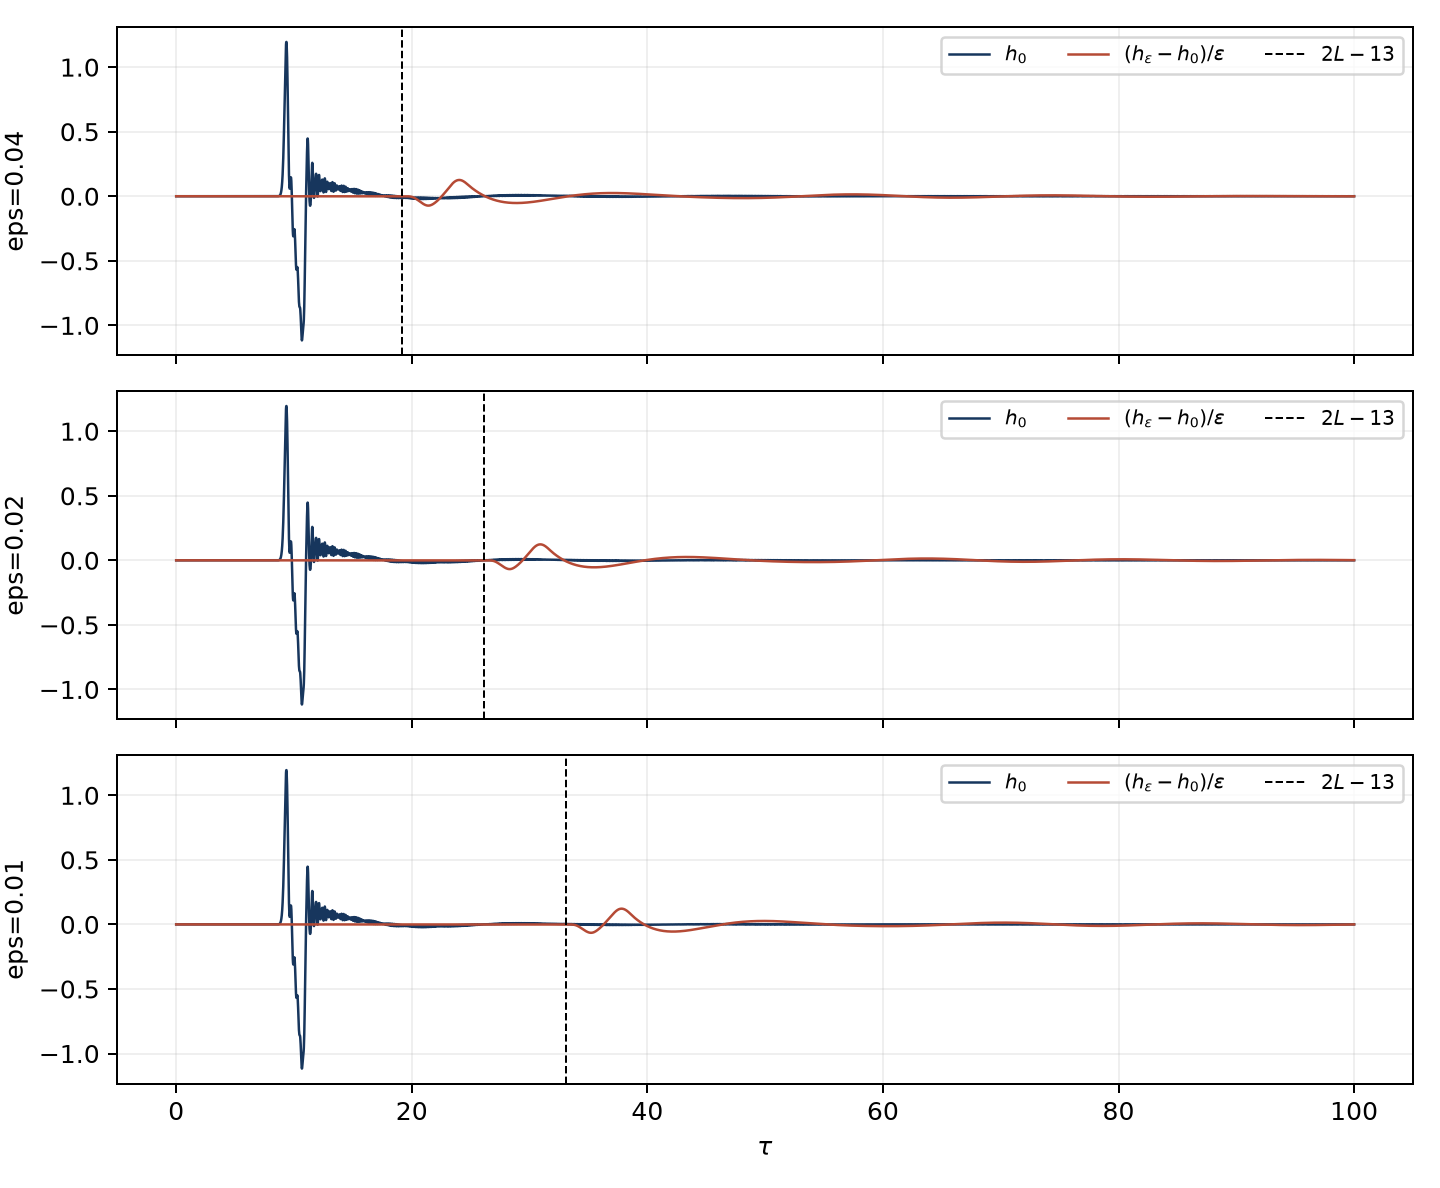
\includegraphics[width=0.68\textwidth]{waveforms_03.png}

\small 图 1：细网格信号。红线为 $(h_\eps-h_0)/\eps$，竖虚线是严格因果时刻
$2L-13$。回波随 $L$ 推迟，而缩放后的首阶波形保持 $O(1)$。
\end{center}

\subsection{频域：外部复标度与直接扰动检验}

在实轴半径 28（复核半径 32）后转入角度 $0.48$ rad、长度 70 的复射线，并沿解析延拓的
$\rho$ 方程积分，避免错误切换 Lambert-$W$ 分支。DOP853 Jost 对数导数匹配得到
\begin{equation}
\om_0=0.373671685104-0.088962316677i.                       \tag{24}
\end{equation}
两半径结果相差 $3.24\times10^{-9}$，Wronskian mismatch 分别为
$9.98\times10^{-11}$ 与 $2.43\times10^{-10}$。

\begin{center}
\small
\begin{tabular}{ccccc}
\toprule
$L$ & $|\partial_\eps\om|$ & $|\partial_\eps\om|e^{-2\gamma L}$ &
$\eps_{\rm chk}$ & 线性预测误差\\
\midrule
12 & 1.02960 & 0.12173 & $10^{-4}$ & $5.84\times10^{-7}$\\
16 & 2.15021 & 0.12478 & $10^{-4}$ & $1.70\times10^{-6}$\\
20 & 4.47857 & 0.12756 & $10^{-4}$ & $8.57\times10^{-6}$\\
\bottomrule
\end{tabular}
\end{center}
第二列约每增加 $\Delta L=4$ 放大 $2.08$ 倍，与
$e^{2\gamma\Delta L}=2.04$ 一致；第三列近似常数。最后一列是直接求扰动后 pole 与
$\om_0+\eps_{\rm chk}\partial_\eps\om$ 的差，显示 $L\mu$ 增大时线性误差同步增大。

\begin{samepage}
\subsection*{复现}
\begin{lstlisting}
python -m pytest -q
python ringdown_stability.py --tmax 100 --coarse-dx 0.08 \
  --fine-dx 0.04 --c 5 --output results_03.json \
  --plot waveforms_03.png
xelatex solution_03.tex
\end{lstlisting}
本次实际运行测试为 \texttt{5 passed}。JSON 保存全部网格、截断尾部、residual 与直接求根数据。
\end{samepage}

\section*{最终回答}

大的 QNM 谱位移与小的有限时间波形误差可以相容。前者由解析延拓中的
$e^{2|\operatorname{Im}\om_0|L}$ 放大，后者先受严格往返延迟 $2L-13$ 限制，并在
$T=O(L)$、$L=c\log(1/\eps)$ 内满足趋零的式 (20)。但是 pole 位置本身没有包含 residue、
source、detector、prompt response 与 branch-cut tail；只有实轴上的 sandwich resolvent
判据 (23) 才能判定全时间观测稳定性。本文已闭合有限窗口结论，但 (Q3c) 的全局版本仍是
明确标记的开放步骤。

\end{document}
